% !TeX spellcheck = en_US
\chapter{Background}%
\label{chap:background}

%%%%%%%%%%%%%%%%%%%%%%%%%%%%%%%%%%%%%%%%%%%%%%%%%%%%%%%%%%%%%%%%%
% Content moved to

\section{The ideal Bose gas within multi-slabs}%
\label{sec:the-ideal-bose-gas-within-a-kronig-penney-potential}

We have studied~\cite{bib:rodriguez-msc-thesis.2014,
	bib:rodriguez-j-low-temp-phys.175.2014,
	bib:rodriguez-j-low-temp-phys.183.2016} the properties of a noninteracting 3D
Bose gas within a periodic potential composed of multiple slabs of width $b$
separated a distance $a$ one from each other. The slabs distribute all over
the space transversely to the $z$ direction, and extend all over the space in
the $x$ and $y$ directions. We model this system through a Kronig-Penny
potential~\cite{bib:kronig-proc-roy-soc-lond.130.1931} in the $z$ direction
composed of potential barriers of width $b$ and separation $a$ with a
magnitude $\vzero$. The period of the potential is $l \equiv a + b$. The magnitude
of the potential determines how probable the tunneling of the bosons through
the barriers is. In the $x$ and $y$ directions we consider that the bosons do
not interact with any external potential so they behave as free particles.
%
\begin{figure}[h!]
	\centering
	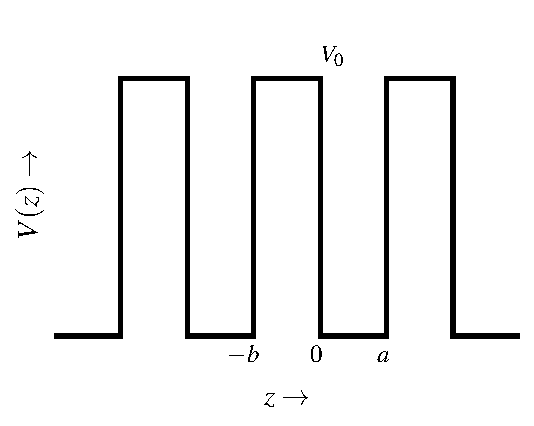
\includegraphics[width=0.6\linewidth]{./figures/kp-potential}
	\caption{Kronig-Penney potential schematic.}\label{fig:kp-potential}
\end{figure}
%

The Schrödinger equation of the system is
%
\begin{equation}
	-\frac{\hbar^2}{2m} \nabla^2 \Psi(\vec r) + \VKP(\vec r) \Psi(\vec r) = \etot \Psi(\vec r),
\end{equation}
%
where $\VKP(\vec r)$ is the {\KP} potential whose definition is
%
\begin{equation}
	\label{eq:kronig-penney-potential}
	\VKP(\vec r) = \begin{cases}
		0   & nl < z < nl + a      \\
		V_0 & nl + a < z < (n+1)l,
	\end{cases}
\end{equation}
%
with $n$ being an integer. As the potential extends all over the space $n$ goes
from $-\infty$ to $\infty$.

Because the bosons that form the gas do not interact between them, the whole
wave function can be decomposed in three components, one for each direction:
%
\begin{equation}
	\Psi(\vec r) \equiv \Psi_x(x) \Psi_y(y) \Psi_z(z).
\end{equation}
%
As a consequence, the total energy is also decomposed in three contributions:
$\ex$, $\ey$, and $\ez$, such that the total energy is the sum of all of them:
$\etot = \ex + \ey + \ez$. As the bosons are free to move in the $x$ and $y$
directions the energy per boson contribution over these axis correspond to that
of the free particle,
%
\begin{equation}
	\ex = \frac{\hbar^2 k_x^2}{2m},  \qquad \ey = \frac{\hbar^2 k_y^2}{2m},
\end{equation}
%
while in the $z$ direction the Schrödinger becomes
%
\begin{equation}
	-\frac{\hbar^2}{2m} \frac{d^2 \Psi_z}{dz^2} + \VKP(z) \Psi_z(z) = \ez \Psi_z(z),
\end{equation}
%
where only appear the component that corresponds to wave function in the $z$
coordinate, $\Psi_z(z)$, and the corresponding energy contribution, $\ez$.

Given that the {\KP} potential $\VKP$ is periodic the solutions of the
differential equation for $\Psi_z(z)$ are Bloch states,
%
\begin{equation}
	\label{eq:bloch-wave}
	\Psi_z(z) \equiv e^{i k_z z} \phi_{k_z}(z),
\end{equation}
%
with $k_z$ being the quasi-momentum of the particles and $\phi_{k_z}(z)$ a
periodic function with the same period of the potential, hence
%
\begin{equation}
	\phi_{k_z}(z + l) = \phi_{k_z}(z).
\end{equation}
%
We solve the Schrödinger equation by applying the boundary conditions of
continuity of the wave function and its derivative, as well as the periodicity
of the wave function. The energy contribution in this direction $\ez$ is then
given by the implicit relation~\cite{bib:kronig-proc-roy-soc-lond.130.1931}
%
\begin{equation}
	\label{eq:kronig-penney-energy}
	\frac{\kappa^2 - \alpha^2}{2 \alpha \kappa} \sinh(\kappa b) \sin(\alpha a) + \cosh(\kappa b) \cos(\alpha a) = \cos \kz(a+b),
\end{equation}
%
where $\hbar\kappa = \sqrt{2m(\vzero - \ez)}$ y $\hbar \alpha = \sqrt{2m\ez}$.
This is the well-known {\KP} dispersion relation.


\subsection{Energy spectrum properties}

As a consequence of the periodic nature of the potential, not all energies in
the $z$ direction are accessible to the particles in the system. We can
understand this directly from eq.~\eqref{eq:kronig-penney-energy}, as only the
right hand side of the equation depends on the momentum of the system $k_z$, and
the left hand side depends only on the energy $\ez$. So, as the right hand side
of the equation is constrained to values within the interval $[-1, 1]$, then
only the values of $\ez$ that make the left hand side to fulfill this constraint
are allowed. This has the consequence that the energy spectrum of the particles
consists of intervals of allowed energies, which we name as energy bands,
separated by regions of energies not allowed, or forbidden bands. The shape of
this bands depends on the potential magnitude $V_0$ and the relation between the
lengths $a$ and $b$.

\begin{SCfigure}
  \centering
  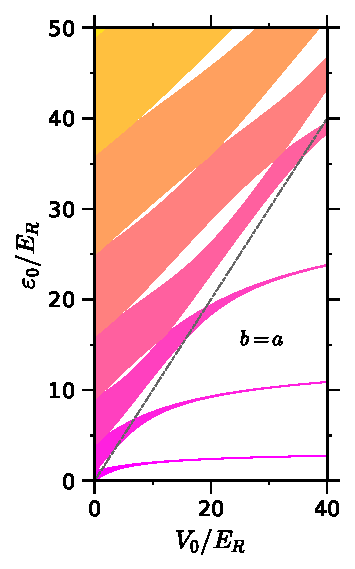
\includegraphics[width=0.6\textwidth]{./figures/energy-spectrum[ideal]_r-1}
	\caption{(Color online) Energy spectrum of a particle within a multi-slabs
  structure as a function of the potential magnitude $\vzero$ (in units of
  $\hbar^2 / 2m(a+b)^2$) for a square lattice $a=b$. The filled regions indicate
  the allowed energy bands of the particle, while the blank regions indicate the
  forbidden bands. The dashed line indicates $\ez = \vzero$. As the potential
  magnitude increases de energy bands become narrower, and for high enough
  potential barriers the bands effectively become energy
  levels.}\label{fig:ideal-energy-per-boson-as-u0-r-1}
\end{SCfigure}

Some results for the energy as a function of the potential magnitude $V_0$ are
shown in the figure~\ref{fig:ideal-energy-per-boson-as-u0-r-1}. In that figure
we can see how the energy spectrum goes from a continuum when $V_0$ is zero,
then it becomes a succession of allowed bands separated by forbidden bands as
$V_0$ increases and then it becomes a series of energy levels when the potential
magnitude becomes large enough.

\subsection{Thermodynamics of the ideal Bose gas}

The thermodynamic properties of the gas such as the internal energy were
obtained from the Grand Thermodynamic Potential $\Omega = U - TS - \mu N$.
From it's differential form we are able to obtain the number of bosons $N$ and
the internal energy $U$, among others properties. In particular, the number
equation allows us to define a criteria to establish when the system presents
the Bose-Einstein condensation phenomena.

In the thermodynamic limit where both number of bosons $N$ and the volume of
the system $V$ go to infinity, but its ratio $N / V$ remains constant, the
energy per particle of the system for nonzero temperatures is given by the
equation
\cite{bib:rodriguez-msc-thesis.2014}
%
\begin{align}
	\label{eq:ideal-internal-energy}
	\nonumber \frac{E}{N} = \ez[0] - \frac{m V}{N (2\pi)^2 \hbar^2} \kbz T & \int_{-\infty}^{\infty} d\kz \; (\ez - \ez[0]) \ln(1 - e^{-(\ez - \mu) / \kbz T}) +                    \\
	                                                                       & \frac{2 m V}{N (2\pi)^2 \hbar^2} (\kbz T)^2 \int_{-\infty}^{\infty} d\kz g_2(e^{-(\ez - \mu)/\kbz T}),
\end{align}
%
where $\kbz$ is the Boltzmann constant, $\mu$ is the chemical potential of the
gas for a given number of bosons and $\ez[0]$ is the ground state energy of the
gas. The right hand side depends on the temperature of the system, both
explicitly and implicitly because of the chemical potential dependence on the
temperature, which is given by
%
\begin{equation}
	\label{eq:ideal-number-of-bosons}
	N = \frac{1}{e^{(\ez[0] - \mu)/\kbz T} - 1} + \frac{m V}{(2\pi)^2 \hbar^2} \kbz T \int_{-\infty}^{\infty} d\kz \; \ln(1 - e^{-(\ez - \mu)/\kbz T}).
\end{equation}
%
The first term of this equation may be interpreted as the number of bosons
occupying the ground state of the system, $N_0(T)$, while the second is the
number of bosons distributed among the excited levels. As we are dealing with a
Bose gas the chemical potential is lower or equal than the ground state
$\ez[0]$, so there is an upper limit for the number of bosons distributed in
excited levels; this limit is reached at a certain temperature $\Tcritic$ when
the chemical potential becomes equal to $\ez[0]$. If the temperature continues
to decrease then the bosons will start to populate massively the ground state,
and the quotient $N_0(T) / N$ may become a significant fraction of the particles
in the gas. The condition at which the $\mu(\Tcritic) \approx \ez[0]$ and the
condensed fraction $N_0(\Tcritic) / N \approx 0$ determines the critical
temperature $\Tcritic$ of Bose-Einstein condensation.

At $T = 0$ the second and thirds terms of~\eqref{eq:ideal-internal-energy}
vanish, and energy per boson becomes effectively $\ez[0]$, the ground state
energy of system.


%%%%%%%%%%%%%%%%%%%%%%%%%%%%%%%%%%%%%%%%%%%%%%%%%%%%%%%%%%%%%%%%%%%%%%%%%%%%%%%%%%%%%%%%%%%%%%

% Contenido movido a mean-field-theory.tex

% \section{The weakly-interacting Bose gas}


%%%%%%%%%%%%%%%%%%%%%%%%%%%%%%%%%%%%%%%%%%%%%%%%%%%%%%%%%%%%%%%%%%%%%%%%%%%%%%%%%%%%%%%%%%%%%%


\section{Lieb-Liniger Bose gas}

There is a many-body quantum system of particular interest: the Lieb-Liniger gas
\cite{bib:lieb-phys-rev.130.1605.1963}. It is a one dimensional Bose gas with
$N$ particles interacting via a contact potential. The Hamiltonian of this
system is
%
\begin{equation}
	\label{eq:lieb-liniger-hamiltonian}
	\qmop{H}_{\mathrm{LL}} = -\frac{\hbar^2}{2m} \sum_{i=1}^{N} \partial^2_{z_i} + g_{1\mathrm{D}} \sum_{i=1}^{N} \sum_{j < k} \delta(z_j - z_k),
\end{equation}
%
where $g_{1\mathrm{D}} = 2\hbar^2 / m \asonedim$ is the strength factor of the
interaction,
%This parameter has been identified by \cite[Olshanni
%1998]{bib:olshanii-phys-rev-lett.81.938} in the study of atomic scattering in a
%gas of impenetrable bosons,
where $\asonedim$ is the effective scattering parameter in one-dimension (see
Sec. \ref{sec:mean-field-theory-in-one-dimension} for further details about the
origin of this parameter).
%\eqref{eq:gross-pitaevskii-interaction-parameter-1d} introduced previously in
%Sec. \ref{sec:the-weakly-interacting-bose-gas}.

The Lieb-Liniger gas is a system that can be solve analytically via a Bethe
ansatz,
%
\begin{equation}
	\psi(z_1, \ldots, z_N) = \sum_{P} a(P) \, e^{i \sum_{j=1}^{N} k_j z_j}.
\end{equation}
%
The wave numbers $k_1, \ldots, k_N$ form an ordered set and the summation
extends over all the permutations $P$ of them, and the coefficient $a(P)$
depends on the permutation. The ground state of the Bose gas at zero temperature
can be expressed as
%
\begin{equation}
	\label{eq:lieb-liniger-energy}
	E =\frac{\hbar^2}{2m} N \densityone^2 e(\gamma(\densityone)),
\end{equation}
%
with $\densityone$ being the average linear density. Unlike the Gross-Pitaevskii
equation, this expression for the energy is valid for all values of
$g_{\mathrm{1D}}$, ranging from the mean-field regime to the Tonks-Girardeau
regime \cite[]{bib:tonks-phys-rev.50.955.1936, bib:girardeau-j-math-phys.1960}.

The function $e(\gamma(\densityone))$ is given by
\cite{bib:lieb-phys-rev.130.1605.1963}
%
\begin{equation}
	\label{eq:lieb-liniger-energy-egamma}
	e(\gamma) = \frac{\gamma^3}{\lambda^3(\gamma)} \int_{-1}^{+1} g(x, \gamma) x^2 \; dx,
\end{equation}
%
with $\gamma = 2 / \densityone \asonedim$. The functions $g$ and $\lambda$ are
determined from the equations
%
\begin{equation}
	\label{eq:lieb-kernel-equation}
	g(x, \gamma) - \frac{1}{2\pi} = \frac{\lambda(\gamma)}{\pi} \int_{-1}^{+1} \frac{g(x', \gamma)}{\lambda^2(\gamma) + (x - x')^2} \; dx'
\end{equation}
%
and
%
\begin{equation}
	\label{eq:lieb-lambda-definition}
	\lambda(\gamma) = \gamma \int_{-1}^{+1} g(x, \gamma) \; dx.
\end{equation}
%
The Eq. \eqref{eq:lieb-kernel-equation} is a Fredholm integral equation of the
second kind (see, e.g., \cite[Chap. 2]{bib:zemyan-fredholm-integral.2012}). This
equation, in conjunction with Eq. \eqref{eq:lieb-lambda-definition} allows us to
find $\lambda$ as a function of $\gamma$ and $g$ as a function of $x$.

Immediately we give a brief description on how to obtain an approximation of the
energy of the ground state \eqref{eq:lieb-liniger-energy}. The method employed
approximates the integrals in equations \eqref{eq:lieb-liniger-energy-egamma},
\eqref{eq:lieb-kernel-equation} and \eqref{eq:lieb-lambda-definition} through a
quadrature rule with $M$ abscissas $x_i$ an its corresponding $w_i$ weights. Any
integral can be approximated through a quadrature as
%
\begin{equation}
	\int_{-1}^{+1} f(x) \, dx \approx \sum_{j=1}^{M} w_j f(x_j).
\end{equation}
%
The accuracy of the approximation will depend on the type of quadrature used.
The abscissas belong to the open interval  $(-1, 1)$ in order to avoid
singularities at the integration limits. Arbitrary integration limits can be
brought to the unit interval through the change of variable $x(t) = (b - a)t/2
	+ (b - a)/2$, hence
%
\begin{equation}
	\int_{a}^{b} f(x) \, dx = \frac{b-a}{2} \int_{-1}^{+1} (f \circ x)(t) \, dt.
\end{equation}
%
We rewrite equation \eqref{eq:lieb-kernel-equation} as
%
\begin{equation}
	\label{eq:lieb-kernel-equation-two}
	g(x, \gamma) - \frac{1}{2\pi} = \frac{\lambda(\gamma)}{\pi} \int_{-1}^{+1} K(x, x') g(x', \gamma) \; dx',
\end{equation}
%
where the kernel of the integral equation is
%
\begin{equation}
	K(x, x') = \frac{\lambda(\gamma)}{\lambda^2(\gamma) + (x - x')^2}.
\end{equation}
%
As a quadrature, Eq. \eqref{eq:lieb-kernel-equation-two} becomes approximately
%
\begin{equation}
	\label{eq:lieb-kernel-equation-quad}
	g(x, \gamma) - \frac{1}{\pi} \sum_{j=1}^{M} w_j K(x, x_j)  g(x_j, \gamma) = \frac{1}{2\pi}.
\end{equation}
%
If we assume that points $g(x_j, \gamma)$ are solutions of
\eqref{eq:lieb-kernel-equation} then for the $i$-nth abscissa $x_i$ the next
equation must hold:
%
\begin{equation}
	\label{eq:lieb-kernel-equation-quad-equation}
	g(x_i, \gamma) - \frac{1}{\pi} \sum_{j=1}^{M} w_j K(x_i, x_j)  g(x_j, \gamma) = \frac{1}{2\pi}.
\end{equation}
%
Considering the whole set of abscissas $x_i$ we have a system of $M$ linear
equations that we can write in matrix notation as
%
\begin{equation}
	\label{eq:lieb-kernel-linear-equation-system}
	\left( \mathbf{I} - \frac{1}{\pi} \mathbf{K} \mathbf{D_w} \right)\mathbf{\tilde{g}} =
	\frac{1}{2\pi} \mathbf{1},
\end{equation}
%
where $\mathbf{\tilde g}$ is the column vector with components $g(x_j)$,
$\mathbf{1}$ is the unit vector, $\mathbf{I}$ is the identity matrix,
$\mathbf{K}$ is the matrix whose $(\mathbf{K})_{ij}$ element is $K(x_i, x_j)$
and $\mathbf{D_w}$ is the diagonal matrix whose diagonal element
$(\mathbf{D_w})_{ii}$ is the weight $w_i$.
%
\begin{figure}[t!]
	\centering
	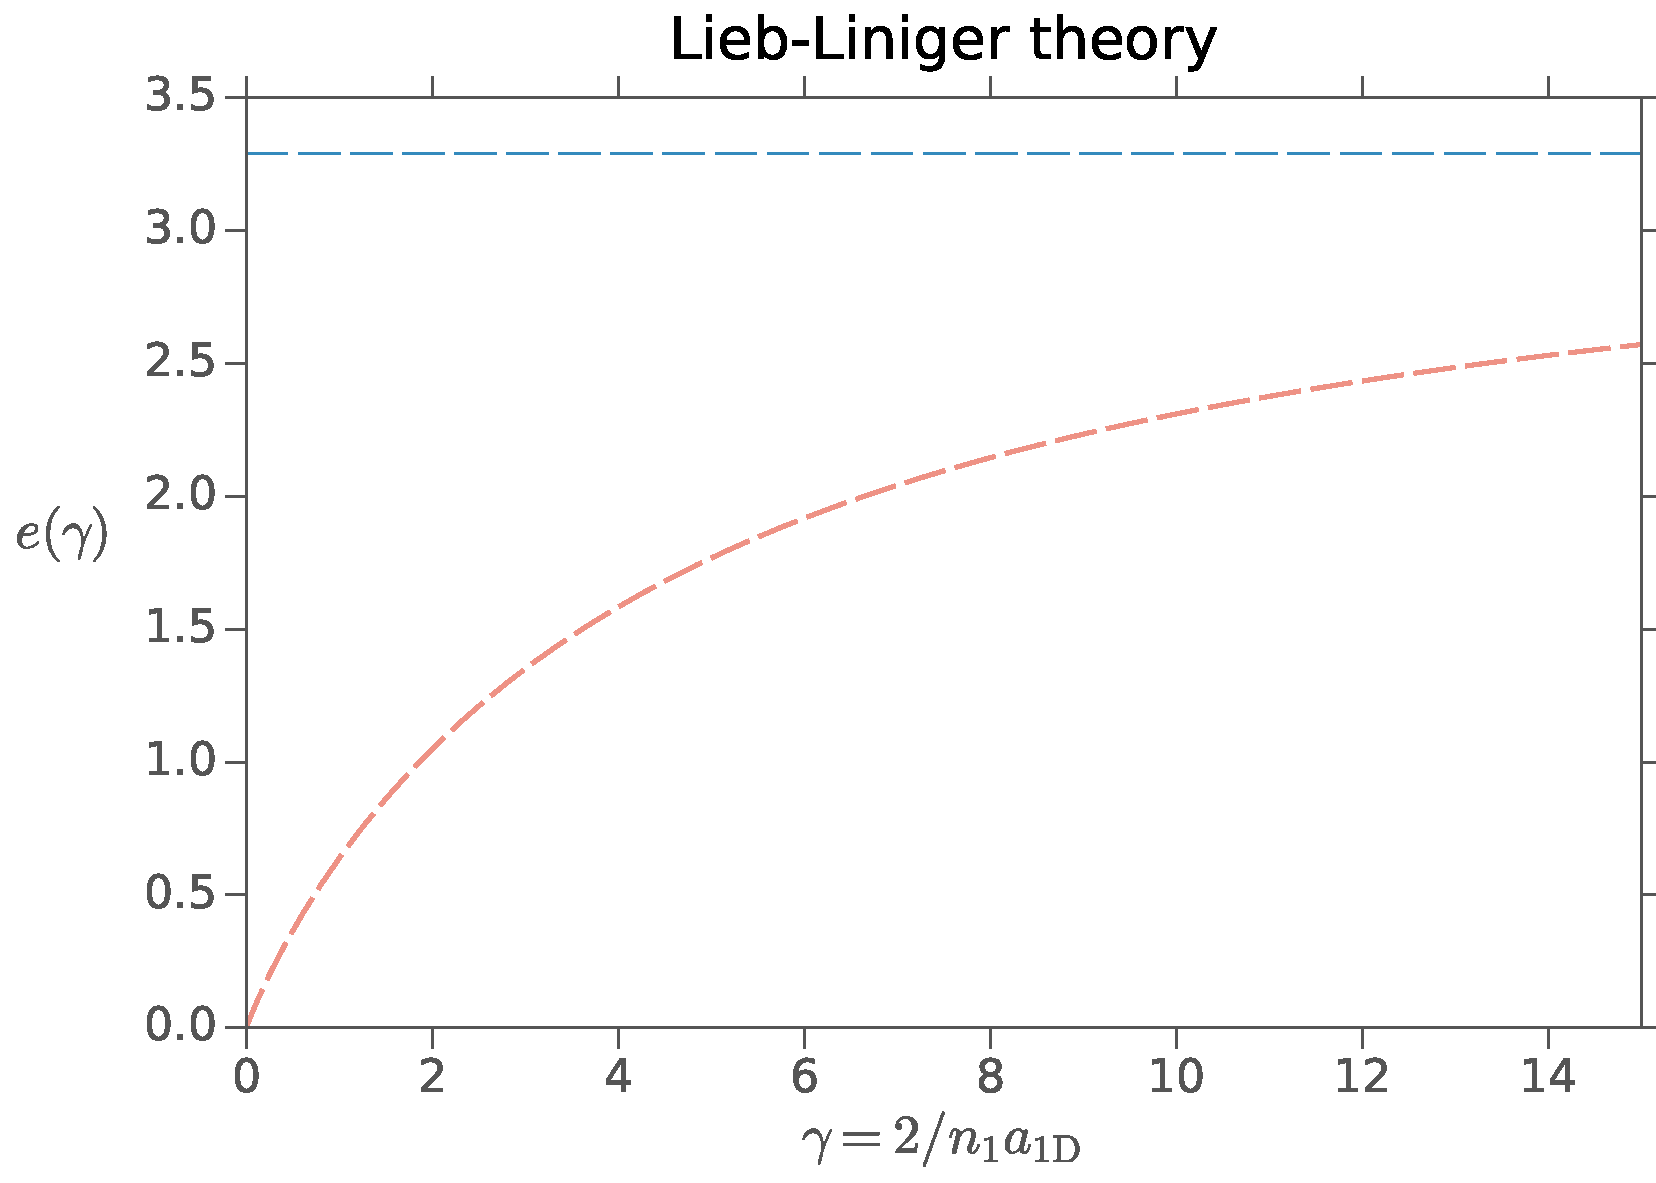
\includegraphics[width=0.85\linewidth]{./figures/lieb-liniger-theory_energy-as-gamma}
	\caption{ Plot of the function $e(\gamma)$ as a function of $\gamma = 2 /
			\densityone \asonedim$ for the Lieb-Liniger theory
		\eqref{eq:lieb-liniger-energy-egamma}. As $\gamma$ increases the function
		tends to the Tonks-Girardeau limit $\pi^2/3$ (dashed horizontal line). }
	\label{fig:lieb-liniger-theory-energy-as-gamma}
\end{figure}
%
The solution of the system \eqref{eq:lieb-kernel-linear-equation-system} for a
fixed value of $\lambda$ give us a set of values $\{ g(x_i) \}$ for a
particular, undetermined $\gamma$. We can use these values together with the
quadrature abscissas and weights in order to calculate the corresponding value
of $\gamma$ through \eqref{eq:lieb-lambda-definition},
%
\begin{equation}
	\gamma \approx \lambda \left( \sum_{j=1}^{M} w_j \, g(x_j) \right)^{-1},
\end{equation}
%
and finally we calculate the function $e(\gamma)$ as
%
\begin{equation}
	e(\gamma) \approx \left(\frac{\gamma}{\lambda}\right)^3 \sum_{j=1}^{M} w_j \, g(x_j) x_j^2.
\end{equation}

%Unlike the Mean-Field theory, the interaction parameter $\gonedim$ can take any
%possible value.
The theory developed by E. H. Lieb and W. Liniger
\cite{bib:lieb-phys-rev.130.1605.1963} examines the behavior of the energy in
the limits when the interaction is very small and when it is too large. In the
high density limit $\densityone \asonedim \gg 1$ the system enters  the
mean-field regime, $\gonedim / \densityone \ll 1$. The Lieb-Liniger theory
yields that $e(\gamma) \approx \gamma$ and the energy per boson is $E/N =
	\hbar^2 \densityone / m \asonedim$, or equivalently, $E/N = \gonedim \densityone
	/ 2$. This result is the same as the one obtained through mean-field theory,
i.e. the Gross-Pitaevskii equation applied to a one-dimensional system, as we
will see in detail in section \ref{sec:mean-field-theory-in-one-dimension}.

In the opposite limit, when $\gonedim / \densityone \gg 1$ the system enters in
the Tonks-Girardeau regime. This is a very important limit as the system behaves
more and more like a gas of impenetrable bosons. In the limit when $\gonedim \to
	\infty$ (impenetrable bosons) the systems manifests the so-called
\textit{fermionization} \cite{bib:girardeau-j-math-phys.1960}, in the sense that
there is a one-to-one correspondence between the wave function of the gas of
impenetrable bosons in one dimension with the wave function of a one-dimensional
gas of noninteracting fermions. The energy of the system becomes independent of
the interaction parameter and it is exactly the same as that of the Fermi gas,
%
\begin{equation}
	\label{eq:tonks-girardeau-energy}
	E = N \frac{\hbar^2 \pi^2 \densityone^2 }{6m}.
\end{equation}
%
The asymptotic behavior of the ground state energy is such that $e(\gamma)
	\rightarrow \pi^2 / 3$.


\section{The weakly-interacting Bose gas in constant potentials}

The behavior and physical properties of a weakly-interacting Bose gas may differ
greatly from the ideal gas even for constant potentials. The study of all these
systems starts from the Gross-Pitaevskii theory (see Sec.
\ref{sec:the-weakly-interacting-bose-gas}), where we solve an equation (the
Gross-Pitaevskii equation) that models the collective behavior of the bosons
that occupy the ground state of the system. Its mathematical form is identical
to the one-body Schrödinger equation with the addition of a nonlinear term
proportional to the square absolute value of the wave function of the condensate
which takes into account the interactions between bosons. It is a widely used
tool to study interacting systems.

Among the solutions to the GP equation one can find localized solutions like
\textit{solitons} in one and three dimensions
\cite{bib:seaman-phys-rev-A.71.033609.2005,
	bib:wang-ying-ying-mod-phys-lett-B.27.12.2013} and even Bloch-wave functions,
i.e, periodic functions with the same period as the potential
\cite{bib:smerzi-phys-rev-E.70.016605.2004}. This solutions may be stable or
unstable depending on whether the interaction is attractive or repulsive, and
depending on the relation between the potential magnitude and the interaction
magnitude. All these solutions are given in terms of the Jacobi elliptic
functions\nocite{bib:abramowitz-stegun-1965}, which are double periodic
functions closely related to the elliptic integrals and can be seen as
generalizations of the circular functions. Although the Gross-Pitaevskii
equation can be solved numerically
\cite{bib:berg-molmer-phys-rev-A.58.1480.1998,
	bib:adhikari-j-of-phys-B.36.12.2003}, these are some of the few systems where
the wave function can be expressed in terms of an analytic function.

To study periodic systems one popular choice is the Dirac-comb potential in one,
two, and three dimensions. This potential is composed by an infinite arrange of
evenly spaced Dirac deltas times a strength factor,
%
\begin{equation}
	\label{eq:dirac-comb-potential}
	V(z) = U_0 \sum_{j=-\infty}^{\infty} \delta(z - j a)
\end{equation}
%
where $V_0$ is the strength factor, $a$ the distance between two consecutive
deltas and $j a$ is the position of the $j$-nth delta. The deltas may extend
over a finite or infinite region of the space with adequate boundary conditions.

The thermodynamics of a 3D noninteracting Bose gas subject to this kind of
potential has been studied extensively
\cite{bib:p-salas-phys-rev-A.82.033632.2010,
	bib:salas-j-low-temp-phys.159.5.2010}, including (but not limited to) the
Bose-Einstein condensation temperature and the heat capacity. For an interacting
system the problem is a lot more difficult even at zero temperature. Mean-field
theory and the Gross-Pitaevskii equation are tools commonly used to study the
properties of these systems such as the energy band spectrum, dynamic stability
and possible phase transitions like superfluidity
\cite{bib:seaman-phys-rev-A.71.033622.2005, bib:dong-laser-physics.17.2.2007}.
It has been found that this potential ---when it extends over the entire
space--- gives rise to stationary solutions in the form of Bloch states with the
same period of the potential, and an energy band structure that resembles that
of the noninteracting case (see figure \ref{fig:seaman-carr-fig-4}). However,
the energy-band shape depends strongly on the magnitude of the interaction
parameter and the trapping potential magnitude, and it may show a very peculiar
behavior identified as \textit{swallowtails} or loop structures that appear at
the edges of the Brillouin zones in the odd bands and at the center of the even
bands. None of these structures appear in the noninteracting case.

%
\begin{figure}[h!]
	\centering
	\fcapside{
		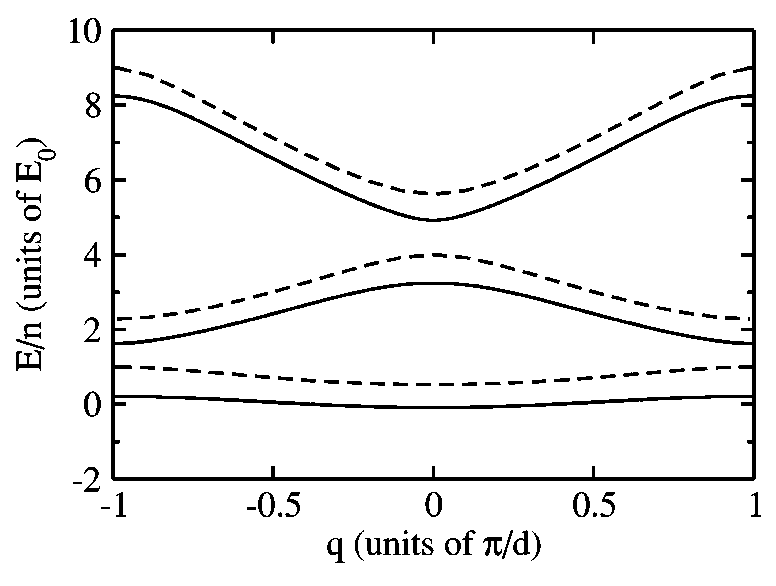
\includegraphics[width=0.95\linewidth]{./figures/seaman-carr-fig-4}
	}{ \caption{ Energy per particle as a function of the quasimomentum wave
			number for the first three bands of a weakly attractive condensate in a
			repulsive lattice generated by a Dirac-comb potential. The noninteracting
			linear band structure is given by the dashed curves
			\cite{bib:seaman-phys-rev-A.71.033622.2005}
			%(Seaman and Carr, Phys. Rev. A. \textbf{71}, 033622 (2005)
			). }
		\label{fig:seaman-carr-fig-4}
	}
\end{figure}

% Aquí falta agregar otra referencia sobre el tema
